\documentclass[twocolumn]{article}
\usepackage[utf8]{inputenc}
\usepackage[margin=1in]{geometry}  % 调整页面边距
\usepackage{titling}               % 控制标题位置
\usepackage{booktabs}              % 表格宏包
\usepackage{amssymb}
% \usepackage{ctex}                  % 中文支持包
\usepackage{authblk}			   % 多作者
\usepackage{graphicx}			% 插入图片设置
\usepackage{tabularx}			% 表格宽度
\usepackage{ragged2e}           % 摘要两端对齐
% \usepackage{xeCJK}
\setlength{\droptitle}{-2.0cm}     % 将标题上移3.0厘米

% \makeatletter
% \def\@date{}  % 完全移除日期
% \makeatother

\title{Medical Image Classification using Support Vector Machine}
\author[1] {DENG Xiaoyu}
\author[1] {TAKAHASHI Yasutake}
% \author[1,3]{Third Author}
\affil[1]{University of Fukui, 3-9-1 Bunkyo, Fukui, 910-0019, Japan}
% \affil[2]{Department of Electrical Engineering, University of Y}
% \affil[3]{Research Institute, Company Z}
\date{2024.11}

\begin{document}

\twocolumn[
	\maketitle

	\begin{center}
		\begin{abstract}
			\begin{justify}
				Support Vector Machines (SVM) are renowned for their efficacy in classification and regression tasks, distinguished by their ability to construct a maximum-margin hyperplane for enhanced model generalization. This study leverages SVM to classify medical images, specifically differentiating between PET and CT lung scans. Utilizing a 928 PET/CT images dataset from the National Cancer Institute’s Cancer Imaging Program, which comprises 251,135 lung scans from 355 subjects, the SVM classifier is trained using hinge loss and optimized via Stochastic Gradient Descent (SGD) with a focus on achieving maximum classification margin. The model's robustness is further enhanced by L2 regularization to prevent overfitting. Preliminary results indicate a high classification accuracy, reaching 100\% on the test set after a complete training cycle, demonstrating SVM's potential in medical image analysis. This research underlines the practical applications of SVM in medical imaging, showcasing its ability to provide precise, reliable classifications.
			\end{justify}
		\end{abstract}
	\end{center}
	\vspace{0.2cm}  % 调整摘要与正文之间的间距
]

\section{Introduction}
Support Vector Machines are a powerful supervised learning algorithm widely used for classification and regression tasks. The algorithm effectively improves model generalization by finding a maximum margin hyperplane in the feature space that distinctly separates different categories.

\section{Related Works}
Support Vector Machines have been applied early on in text classification tasks, such as spam detection and web page categorization \cite{hearst_support_1998}. In fields like face recognition, handwriting recognition \cite{bahlmann_online_2002}, and medical image analysis \cite{gautam_investigation_2021}, SVM has been widely used due to its efficient classification capabilities. The development and application of SVMs are a success story in the field of machine learning, showcasing how theoretical research can be transformed into effective practical tools.

\section{Method}
The goal of this study is to utilize Support Vector Machines for classification tasks, aiming to find a decision boundary, i.e., a hyperplane that maximally separates different categories of data points. The hyperplane can be expressed as:
\[
	f(x) = \mathbf{W}^\mathbb{T} x + b
\]
where \(f(x)\) is the model's predictive output, indicating the confidence level of sample \(x_i\) belonging to a specific category. \( \mathbf{W} \) is the normal vector to the hyperplane, \( b \) is the bias term, and \( x \) is the input feature vector.

SVM optimizes \( \mathbf{W} \) and \( b \) by solving an optimization problem aimed at maximizing the margin between two categories. The classifier is typically trained using the hinge loss, which encourages finding a decision boundary with the maximum margin, defined as:
\[
	L(y_i, f(x_i)) = \max(0, 1 - y_i f(x_i))
\]
where \( f(x_i) = \mathbf{W}^\mathbb{T} x_i + b \) and \( y_i \) are the actual class labels, with values \{-1, 1\}. This study constructs a basic SVM, optimized using hinge loss, to implement a medical image classifier.

\section{Experiments}
This study applies SVM to classify medical images, distinguishing between PET and CT images. The dataset originates from the National Cancer Institute's Cancer Imaging Program (CIP), covering 251,135 lung scans from 355 subjects \cite{li_large-scale_2020}. These scans were primarily collected between 2009 and 2011, with each subject's data including gender, age, weight, smoking history, and cancer diagnosis classification. All scan data are stored in DICOM format. For this experiment, data from 38 subjects diagnosed with small-cell lung cancer were selected, including PET scans, various CT scans, and fusion-enhanced scan images, totaling 12,930 images. Through precise selection, 928 scan images were obtained for use in this study.

These 928 PET/CT lung scan images are used for this study. The data partitioning in this experiment is shown in Table \ref{tab:dataset_partition_1}.

% Insert data partition table
% \begin{table}[h]
% 	\centering
% 	\caption{Experiment Data Partition}
% 	\label{tab:dataset_partition_1}
% 	\begin{tabular}{ccc}
% 		\toprule
% 		Parameter Count & Testing & Training \\
% 		\midrule
% 		Lung PET & 24 & 440 \\
% 		Lung CT & 24 & 440 \\
% 		Total & 48 & 880 \\
% 		\bottomrule
% 	\end{tabular}
% \end{table}

\begin{table}[h]
	\centering
	\caption{Experiment Data Partition}
	\label{tab:dataset_partition_1}
	\begin{tabularx}{\linewidth}{X c c}
		\toprule
		Parameter Count & Testing & Training \\
		\midrule
		Lung PET        & 24      & 440      \\
		Lung CT         & 24      & 440      \\
		Total Images    & 48      & 880      \\
		\bottomrule
	\end{tabularx}
\end{table}

The number of parameters that need to be optimized in the decision function, built for different sizes of input images, is listed in Table \ref{tab:params_count}. The 464 pairs of PET/CT lung scan data were exported as 256×256 pixel RGB format PNG images. Thus, the decision function needs to construct an input data column vector of dimensions $256 \times 256 \times 3 = 196608$, hence $\mathbf{W}^\mathbb{T}$ should be a row vector of $196608$ and $1$ bias term $b$.

% Insert parameter count table
\begin{table}[h]
	\centering
	\caption{Number of Parameters to be Optimized in SVM Decision Functions for Different Input Image Sizes}
	\label{tab:params_count}
	\begin{tabular}{cccc}
		\toprule
		Parameters & 128×128 & 256×256 & 512×512 \\
		\midrule
		Channel=1  & 16,385  & 65,537  & 262,145 \\
		Channel=2  & 32,769  & 131,073 & 524,289 \\
		Channel=3  & 49,153  & 196,609 & 786,433 \\
		\bottomrule
	\end{tabular}
\end{table}

This experiment employs a standard Support Vector Machine (SVM) classifier to categorize positron emission tomography (PET) and computed tomography (CT) images. The hinge loss, used as the standard loss function for SVM classification, is chosen due to its excellent performance in maximizing the margin in classification problems. The model optimization algorithm uses Stochastic Gradient Descent (SGD), with a learning rate (lr) set at 0.001. This relatively low learning rate helps the model to stably approach the global optimum during training.

% Insert loss and accuracy charts
\begin{figure}[h]
	\centering
	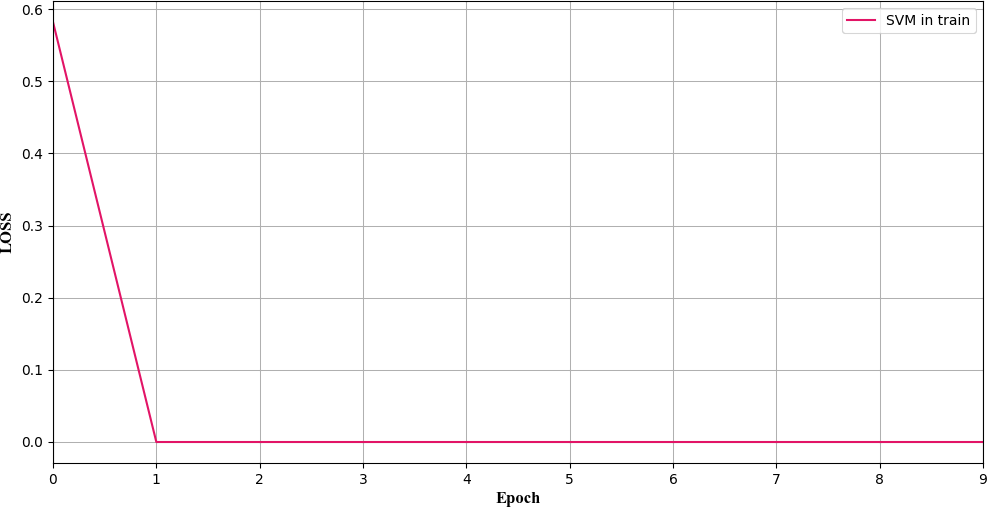
\includegraphics[width=1.0\linewidth]{exp_log/train440_valid024/LOSS_train}
	\caption{Loss Curve Across All Epochs in Training Process}
	\label{fig:loss_train}
\end{figure}

\begin{figure}[h]
	\centering
	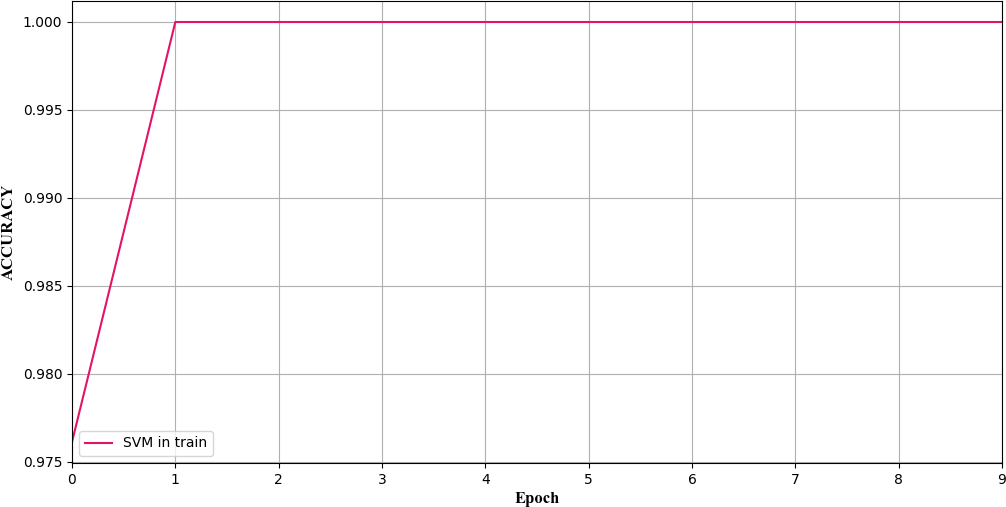
\includegraphics[width=1.0\linewidth]{exp_log/train440_valid024/ACCURACY_train}
	\caption{Accuracy Curve Across All Epochs on Training Set}
	\label{fig:acc_train}
\end{figure}

To enhance the model's generalization capability and mitigate overfitting issues, L2 regularization is applied, setting the weight decay parameter to 0.001. Multiple training epochs were recorded, including data on loss values, the number of correctly classified samples, total number of samples, and classification accuracy, as shown in Figure \ref{fig:loss_train}. The x-axis represents the training epochs, and the y-axis represents loss values as classification accuracy.
Figures \ref{fig:acc_train} and \ref{fig:acc_test} show the classification accuracy on the training and test sets, respectively, on their y-axes.
Notably, by the end of the first training epoch, the accuracy had reached a significantly high level, indicating that the training data was sufficient, and SVM was able to competently handle the classification tasks on this dataset after just one training cycle.

\begin{figure}[h]
	\centering
	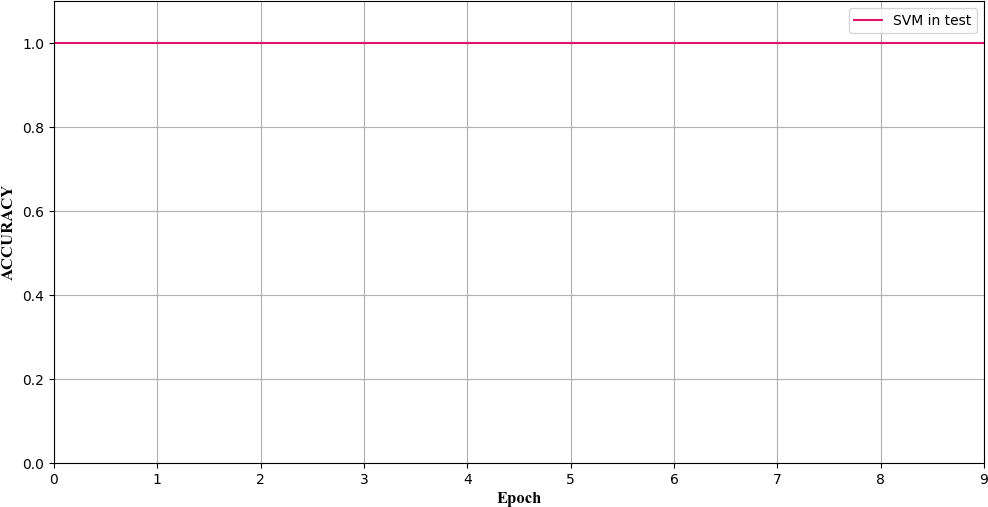
\includegraphics[width=1.0\linewidth]{exp_log/train440_valid024/ACCURACY_test}
	\caption{Accuracy Curve Across All Epochs on Test Set}
	\label{fig:acc_test}
\end{figure}

To detail the optimization during the first cycle, we have created Figure \ref{fig:acc_train_e0}, where the x-axis represents the number of training batches, and the y-axis shows the accuracy of SVM after gradient descent training in prior batches. The experimental results show that the SVM classifier had an initial training accuracy of 50\%.
After a complete training cycle, the model achieved a classification accuracy of 100\% on the test set. This may also be attributed to the relatively small size of the training dataset.

\begin{figure}[h]
	\centering
	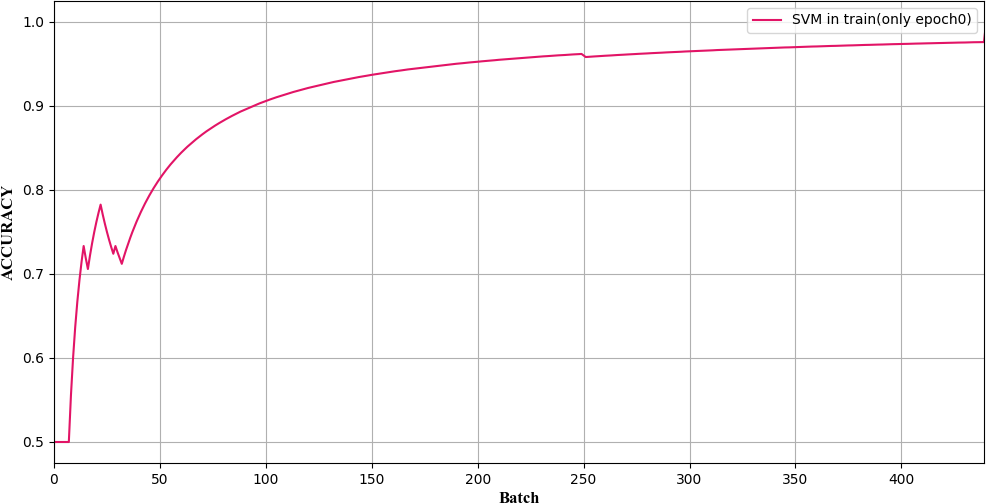
\includegraphics[width=1.0\linewidth]{exp_log/train440_valid024/ACCURACY_train_epoch0}
	\caption[acc_train_e0]{Accuracy Line Figure in Epoch 0 in Train Process}
	\label{fig:acc_train_e0}
\end{figure}

\section{Conclusion}
This study extensively explores the historical development, technical principles, and practical applications of Support Vector Machines, particularly in medical image classification tasks. The experimental results demonstrate that training and testing SVM on this dataset not only effectively accomplishes the classification task but also exhibits excellent classification performance.

\section*{Acknowledgements}
This paper expresses its gratitude to the National Cancer Institute's Cancer Imaging Program, which has generously made its high-quality medical imaging dataset available and authorized for use on the internet, providing invaluable resources for the smooth conduct of this research.


\bibliographystyle{unsrt}
\bibliography{svm}

\end{document}
